\section{Soft- und Hardware}
\label{sec:softundhardware}
%==============================================================================

Im Folgenden werden die wichtigsten Konzepte näher erläutert.

\subsection{Microsoft Kinect}
\label{subsec:kinect}
{\color{red}Auflösung, Reichweite, Genauigkeit in Abhängigkeit zur Entfernung, generelle Funktionsweise, schatten nicht vermeidbar(aussage wird referenziert)}
{\color{red}openni\_kinect stack erwähnen/referenzieren!}
{\color{red}Überleitung zu ROS, wir brauchen ROS!}

\subsection{Robot Operating System}

\gls{ROS} ist ein Open-Source Betriebssystem, welches viele Probleme und Aspekte verteilter, komplexer Software bezüglich der Anwendungsentwicklung für Roboter kapselt. Falls nicht anders gekennzeichnet, dient \cite{Quigley:2009kx} in diesem Abschnitt als Quelle.

Im eigentlichen Sinne ist \gls{ROS} kein Betriebssystem. Vielmehr handelt es sich um ein leichtgewichtiges C++ Framework, das in einem bestehenden Betriebssystem ausgeführt wird. Dabei verwendet es eine Peer-to-peer Kommunikationsarchitekur, mit Hilfe derer einzelne Programme in verschiedenen Programmiersprachen unabhängig voneinander kommunizieren können. \gls{ROS} legt zudem großen Wert auf eine Tool-basierte Funktionsweise. Das heißt, dass alles strikt in Module gegliedert ist, wodurch das Framework selbst sowie die einzelnen Module besonders gut getestet werden können.

In dieser Arbeit dient \gls{ROS} als eine robuste Architektur zum Transport verschiedener Daten zwischen Programmen, die bei Bedarf auch auf verschiedenen Computern im Netzwerk ausgeführt werden können. Wie in den Kapiteln \ref{sec:pathfinder} und \ref{sec:navstack} näher beschrieben, bietet \gls{ROS} bereits einen großen Funktionsumfang bezüglich des Umgangs mit Robotern. Im Folgenden wird eine kurze Einführung in die generelle Architektur sowie in in dieser Arbeit benötigte Tools gegeben.

\subsubsection{Architektur}

Einzelne Module beziehungsweise Programme in einer \gls{ROS} Umgebung werden \glspl{glos:Node} bezeichnet. Diese können beliebg oft unter Angabe eines Namensraumes gestartet werden. Das heißt ein \gls{glos:Node} kann generisch Aufgaben lösen, ohne zu wissen, ob er beispielsweise gerade den rechten oder linken Arm eines Roboters repräsentiert.

Damit ein \gls{glos:Node} unter \gls{ROS} übersetzt beziehungsweise ausgeführt werden kann, muss er einem \gls{glos:Package} zugeordnet sein. Ein \gls{glos:Package} kann mehrere \glspl{glos:Node} beinhalten. Es definiert durch eine \gls{glos:Manifest} Datei, welche Abhängigkeiten es zu anderen \glspl{glos:Package} besitzt. Mehrere \glspl{glos:Package} können zu einem \gls{glos:Stack} zusammengeschlossen sein, beispielsweise wenn sie eine gemeinsame Aufgabe erfüllen, indem sie diese in Teilaspekte zerlegen. Ein solcher \gls{glos:Stack} besitzt dann ebenfalls ein \gls{glos:Manifest}.

Innerhalb der \glspl{glos:Package} oder \glspl{glos:Stack} können \glspl{glos:LaunchFile} angelegt werden, die das Starten eines ganzen Systems mit mehreren \glspl{glos:Node} erleichtern. Dabei kann in einer solchen Datei auch definiert sein, dass bestimmte \glspl{glos:Node} nicht lokal, sondern entfernt auf einem anderen Computer gestartet werden. Außerdem können hier Parameter an die \glspl{glos:Node} übergeben werden, die sich üblicherweise nur selten ändern. \glspl{glos:LaunchFile} können zudem andere \glspl{glos:LaunchFile} rekursiv inkludieren und dabei auch Parameter überschreiben{\color{red} (Inernet-)Quelle dafür angeben, da nicht in angegebener Quelle)}. Verzichtet man auf eine \gls{glos:LaunchFile}, dann müssen die \glspl{glos:Node} einzeln gestartet und auch wieder beendet werden. Durch die \gls{glos:LaunchFile} können alle gestarteten \glspl{glos:Node} über STRG+C zusammen beendet werden.

\glspl{glos:Node} kommunizieren über das \gls{ROS} interne Kommunikationsnetzwerk miteinander. Das heißt, wenn ein \gls{glos:Node} Informationen anderen \glspl{glos:Node} zur Verfügung stellt, veröffentlicht er diese über ein bestimmtes \gls{glos:Topic}. Andere \glspl{glos:Node} können dieses \gls{glos:Topic} abonnieren. Dabei haben \glspl{glos:Topic} immer einen bestimmten Namen, der sowohl durch \glspl{glos:Node}, die Informationen veröffentlichen, als auch von \glspl{glos:Node} die Informationen abonnieren, die sie benötigen um ihre Funktionalität zu erfüllen, festgelegt sein kann. Um einen Konflikt zu vermeiden, muss in einem konkreten System in der \gls{glos:LaunchFile} eine Abbildung zwischen \gls{glos:Topic} Benennungen stattfinden. \glspl{glos:Node} können zudem sehen, ob ihr eigenes \gls{glos:Topic} abonniert wurde. Dadurch lässt sich Rechenzeit sparen, sollte kein Abonnent vorhanden sein.

Informationen werden in \glspl{glos:Message} zu einem \gls{glos:Topic} veröffentlicht. Sie werden zunächst in einer platformunabhängigen Sprache definiert, einer \gls{IDL}. Diese Abstraktion erlaubt es, in wenigen Zeilen eine \gls{glos:Message} zu definieren. Entsprechende Code Generatoren in verschiedenen Sprachen erzeugen automatisch aus dieser Definition Klassen, welche durchaus hunderte Zeilen Code umfassen können. Dadurch fällt es dem Programmierer sehr viel einfacher, in \gls{ROS} sprachenunabhängig neue zuvor nicht bekannte \glspl{glos:Message} zu definieren. Viele oft benötigte \glspl{glos:Message} werden beispielsweise bereits durch den \emph{common\_msgs} \gls{glos:Stack} zur Verfügung gestellt. Zusätzlich zur \gls{glos:Topic} Architektur gibt es in \gls{ROS} \glspl{glos:Service}, welche einen optionalen Parameter erhalten, und üblicherweise einen Rückgabewert liefern. Durch diese kann eine synchrone Kommunikation zwischen \glspl{glos:Node} stattfinden. 

\subsubsection{Tools}

{\color{red}Quellen finden!}

Ein \gls{glos:Package} wird über das Tool \emph{rosmake PACKAGE\_NAME} kompiliert. Dabei werden falls nötig alle Abhängigkeiten die in der \gls{glos:Manifest} Datei eingetragen wurden ebenfalls rekursiv kompiliert. Ein \gls{glos:Package} mit mehreren \glspl{glos:Node} besitzt somit mehrere ausführbare Dateien, die über \emph{rosrun PACKAGE\_NAME NODE\_NAME} einzeln, über \emph{roslaunch PACKAGE\_NAME LAUNCH\_DATEI\_NAME} zusammen, gestartet werden.

Damit gestartete \glspl{glos:Node} sich in \gls{ROS} finden, gibt es einen Namensdienst, den sogenannten Master. Alle \glspl{glos:Node} melden sich an diesem Dienst an, und erhalten hierüber Direktverbindungen zu anderen \glspl{glos:Node}. Dieser Dienst wird entweder über die Konsole mit dem Befehl \emph{roscore}, oder implizit durch Benutzung einer \gls{glos:LaunchFile} gestartet. Ein spezieller \gls{glos:Node} namens \emph{rosout} wird immer gemeinsam mit dem Master gestartet. Er bekommt automatisch Log Nachrichten aller \glspl{glos:Node}. Diese können an zentraler Stelle mit dem Tool \emph{rxconsole} angezeigt werden.

Da eine Topographie mit vielen \glspl{glos:Node} sehr unübersichtlich sein kann, bietet \gls{ROS} ein Tool namens \emph{rxgraph} an. Dieses Tool zeigt alle \glspl{glos:Node} visuell als Knoten und verbindet diese, sollten sie \glspl{glos:Topic} einander abonnieren.

Um einzelne \glspl{glos:Node} oder ein ganzes System zu testen, kann es sinnvoll sein, bestimmte Daten beispielsweise einer Kamera oder eines Roboters, bei einem normalen Test aufzunehmen und anschließend so wieder abzuspielen, dass der eigene noch zu entwickelnde \gls{glos:Node} mit diesen Daten als Eingabe getestet werden kann. \gls{ROS} stellt hierfür das Tool \emph{rosbag} zur Verfügung. Mittels \emph{rosbag record TOPIC\_NAME(N) -O DATEI} werden ein oder mehrere \glspl{glos:Topic} abonniert und in einer einzelnen Datei aufgezeichnet. Über \emph{rosbag play DATEI(-EN)} werden eventuell mehrere solche Dateien gleichzeitig wieder abgespielt. Dabei werden die Zeitstempel beachtet, die in einer jeden aufgezeichneten \gls{glos:Message} enthalten sind. Die Reihenfolge, in der die \glspl{glos:Message} während des Aufzeichnens erstellt wurden, entspricht also auch der Abspielreihenfolge.

\glspl{glos:Message} transportieren üblicherweise Daten, die visualisiert werden können. \gls{ROS} hält hierfür einen \gls{glos:Node} namens \gls{glos:rviz} bereit. Dieser versteht bereits einige \glspl{glos:Message}, kann aber auch bei Bedarf durch Plug-Ins erweitert werden. In dieser Arbeit wird \gls{glos:rviz} beispielsweise dafür eingesetzt, eine Karte und einen Roboter darin anzuzeigen. Hierbei wird deutlich, dass \gls{glos:rviz} die Transformation zwischen Karte und Roboter kennen muss. Dafür sorgt ein sehr wichtiges \gls{glos:Package} namens \emph{tf}. Jede \gls{glos:Message} ist in einem bestimmten Koordinatensystem entstanden, einem sogenannten \gls{glos:CFrame}, welcher in einer \gls{glos:Message} durch einen String repräsentiert wird. Der \emph{tf}-\gls{glos:Node} abonniert nun alle \emph{tf-\glspl{glos:Message}}, die zu einem \gls{glos:Topic} namens \emph{/tf} beispielsweise von Sensoren veröffentlicht werden. Andere \glspl{glos:Node}, die die Transformation zwischen zwei \glspl{Frame} benötigen, wie beispielsweise \gls{glos:rviz} zum Visualisieren der \glspl{glos:Message}, können nun anhand der gesammelten Daten des \emph{tf-\glspl{glos:Node}} diese direkt ablesen. Diese Transformationen werden in einer Baumstruktur vorgehalten. Es muss also zwischen zwei \glspl{Frame} immer genau eine Hierarchie geben. In \gls{glos:rviz} selbst, kann der Anwender einen globalen \gls{glos:FFrame} wählen, in den alle sonstigen \glspl{Frame} unter Beachtung ihrer Transformation zu diesem gezeichnet werden, typischerweise also die Wurzel des \emph{tf}-Baumes. Zusätzlich lässt sich ein \gls{glos:TFrame} auswählen, den der Benutzer verfolgen möchte. Wird also eine Karte als \gls{glos:TFrame} gewählt, bewegt sich der Roboter. Wird der Roboter selbst ausgewählt, bewegt sich die Karte während der Roboter immer in der Mitte bleibt.

\subsection{OpenNI\_Kinect Stack}

Der OpenNI\_Kinect Stack integriert unter Anderem die in \ref{subsec:kinect} beschriebene Kinect in \gls{ROS}. Er erlaubt neben Skeleton Tracking und Gesture Recognition auch die direkte Verwendung der Rohdaten der \gls{glos:Kinect} durch das \gls{glos:Package} \emph{openni\_camera}. Wie in \cite{online:rosopenni_camera} beschrieben, werden durch das Starten des \emph{openni\_camera} \glspl{glos:Node} u. a. die in der Tabelle \ref{tab:opennicameramsgs} {\color{red} (steht hier immer noch ein doppeltes fragezeichen?)} beschriebenen \glspl{glos:Message} zu den jeweiligen \glspl{glos:Topic} veröffentlicht.
\begin{table}
\label{tab:opennicameramsgs}
\begin{tabular}{ l l p{4.3cm} }
	\hline
	\gls{glos:Message}			&	\gls{glos:Topic}						& 	Beschreibung\\
	\hline
	sensor\_msgs/CameraInfo		&	/camera/depth/camera\_info			&	Parameter der Infrarot Kamera\\
	stereo\_msgs/DisparityImage	&	/camera/depth/disparity				&	{\color{red}was ist das, brauchen wir das?}\\
	sensor\_msgs/Image			&	/camera/depth/image					&	Tiefenbild, enthält die Entfernungen in Metern\\
	%sensor\_msgs/CompressedImage	&	/camera/depth/image/compressed		&	\\
	%sensor\_msgs/Image			&	/camera/depth/image\_raw				&	\\
	%sensor\_msgs/CompressedImage	&	/camera/depth/image\_raw/compressed	&	\\
	sensor\_msgs/PointCloud2		&	/camera/depth/points					&	farblose \gls{glos:Pointcloud}\\
	\hline
	sensor\_msgs/CameraInfo		&	/camera/rgb/camera\_info				&	Paramter der RGB Kamera\\
	sensor\_msgs/Image			&	/camera/rgb/image\_color				&	RGB Bild\\
	%sensor\_msgs/CompressedImage	&	/camera/rgb/image\_color/compressed	&	\\
	sensor\_msgs/Image			&	/camera/rgb/image\_mono				&	Bild in Graustufen\\
	%sensor\_msgs/CompressedImage	&	/camera/rgb/image\_mono/compressed	&	\\
	%sensor\_msgs/Image			&	/camera/rgb/image\_raw				&	\\
	%sensor\_msgs/CompressedImage	&	/camera/rgb/image\_raw/compressed		&	\\
	sensor\_msgs/PointCloud2		&	/camera/rgb/points					&	farbige \gls{glos:Pointcloud}\\
	\hline
\end{tabular}
\caption[Topic-Übersicht von openni\_camera]{Übersicht der veröffentlichten Informationen von \emph{openni\_camera}.}
\end{table}
Über jeweils einen \gls{glos:Service} \emph{set\_camera\_info} erlaubt das \gls{glos:Package} zusätzlich eine Konfiguration und Kalibrierung der Infrarot und RGB Kamera.

Eine \gls{glos:Message} des Typs \emph{PointCloud2} wird hierbei dazu verwendet, 3D Informationen zu veröffentlichen\footnote{siehe \ref{table:opennicameramsgs}}. Diese \gls{glos:Message} besitzt wie in \cite{online:pointcloud2} näher beschrieben u.a. folgende Komponenten:

\begin{description}
	\item[Header]		Sequenznummer, Zeitstempel und Informationen über den \gls{glos:CFrame}
	\item[Fields]		Liste aller Felder eines Punktes
	\item[Row\_Step]	Länge einer Zeile
	\item[Data]		Liste aller Punkte
\end{description}

In Abbildung \ref{fig:kinectViews} sind zwei solche \glspl{glos:Pointcloud} aus zwei verschiedenen Winkeln dargestellt. Auf der linken Seite ist nahezu die Sicht der \gls{glos:Kinect} zu sehen, während auf der rechten Seite der Sichtwinkel auf die Wolke stark geändert wurde. Beide Bilder wurden zu unterschiedlichen Zeiten aufgenommen, ohne die Position der \gls{glos:Kinect} zu verändern. Dadurch ist ein unterschiedliches Rauschen an den Rändern der Farbbereiche gut zu erkennen.

{\color{red}Farbbereiche-Entfernungen erklären}

\begin{figure}[t]
	\centering
	\fbox{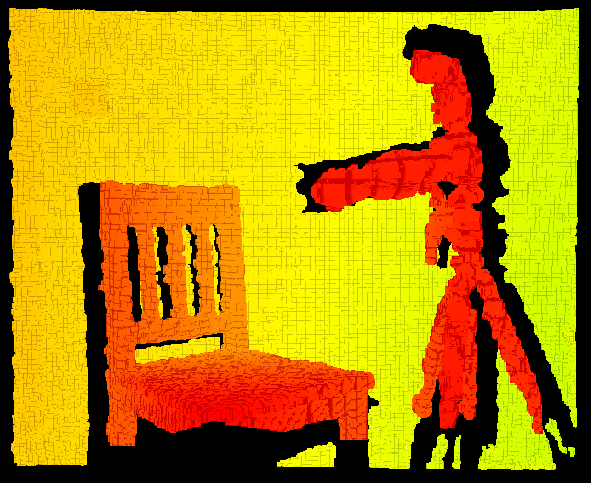
\includegraphics[height=6.5cm]{./graphics/kinectFrontView}}
	\fbox{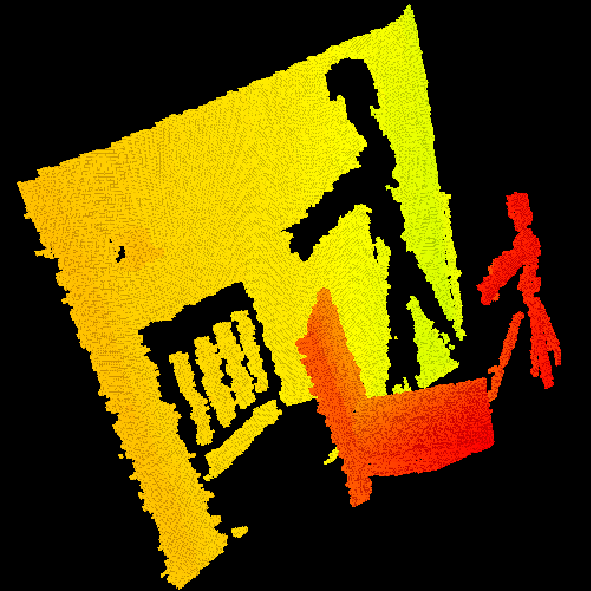
\includegraphics[height=6.5cm]{./graphics/kinectSideView}}
	\caption[Kinect Pointcloud]{Zwei \glspl{glos:Pointcloud} der \gls{glos:Kinect}, visualisiert durch \gls{glos:rviz}.}
	\label{fig:kinectViews}
\end{figure}

\subsection{Turtle Bot}
{\color{red}lorem ipsum!}